\section{Approach}
\label{sec:approach}

This section presents our methodology for systematically generating adversarial scenarios to evaluate autonomous driving systems. Our approach has the following workflow: Sec.~\ref{sec:typology_selection} selects and justifies ten target pre-crash typologies from the NHTSA classification, grouped into three kinematic categories. Sec.~\ref{sec:threshold_selection} then establishes a two-tier threat metric framework, with threshold values derived from Euro~NCAP protocols, that provides the quantitative criteria for identifying seed scenarios and evaluating generated candidates. Finally, Sec.~\ref{sec:generation} details the adversarial generation pipeline itself, which transforms real-world near-miss events into analytically more critical test cases through parameterized perturbation, open-loop analytical optimisation, and diversity-driven selection.
\subsection{Target Pre-Crash Typology Selection}\label{sec:typology_selection}
\begin{figure}
    \centering
    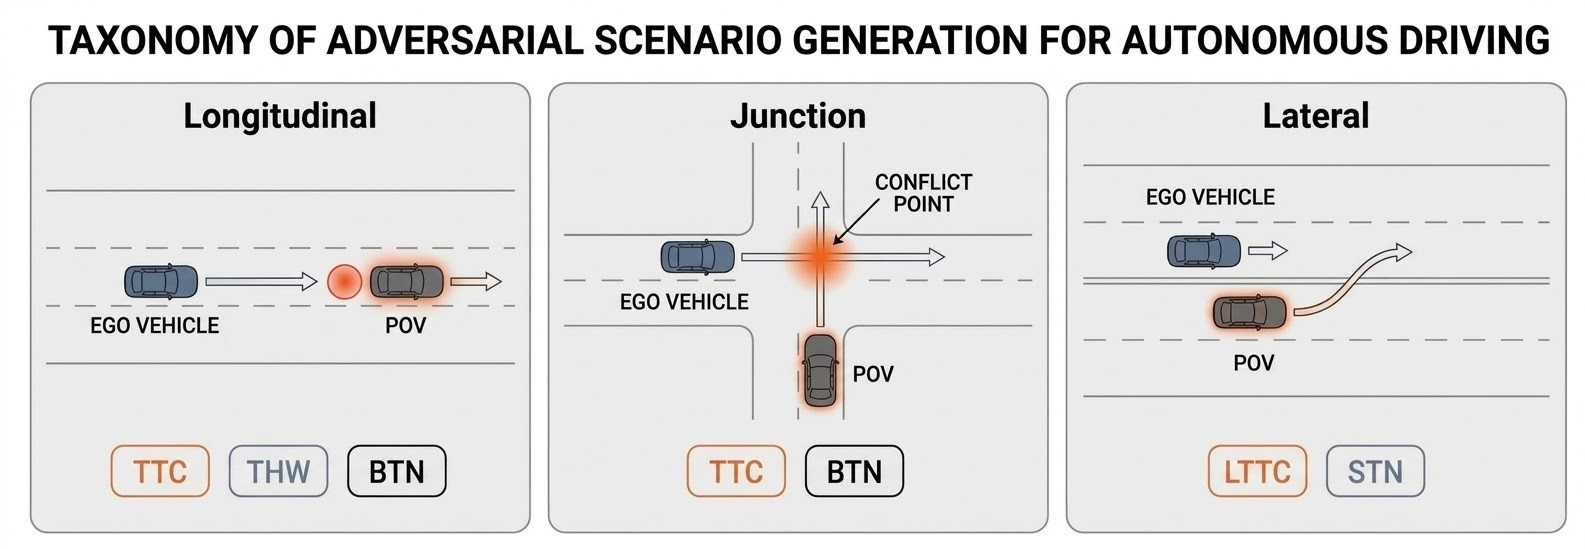
\includegraphics[width=\linewidth]{figures/scenario_taxonomy.png}
    \caption{Visual taxonomy of the three kinematic categories, their spatial configurations, associated threat metrics, and adversarial generation strategies.}

    \label{fig:scenario_taxonomy}
\end{figure}
\begin{table*}[t]
  \caption{Categorization of NHTSA Pre-Crash Scenarios and Target Threat Metrics}
  \label{tab:kinematic_categories}
  \renewcommand{\arraystretch}{1.0} 
  \begin{tabularx}{\textwidth}{@{} 
      >{\hsize=0.25\hsize\raggedright\arraybackslash}X 
      >{\hsize=0.50\hsize\raggedright\arraybackslash}X 
      >{\hsize=0.25\hsize\raggedright\arraybackslash}X 
      @{}}
    \toprule
    \textbf{Kinematic Category} & \textbf{Included Typologies (NHTSA)} & \textbf{Target Metrics} \\
    \midrule
    
    \rowcolor{blue!5}
    \textbf{Longitudinal} & 
    (1) Lead Vehicle Stopped \newline 
    (2) Lead Vehicle Decelerating \newline 
    (3) Lead Veh. Moving at Lower Speed & 
    TTC, THW, BTN \\
    
    \rowcolor{green!5}
    \textbf{Junction} & 
    (4) Veh. Turning at Non-Signalized \newline 
    (5) Straight Crossing Non-Signalized \newline 
    (6) LTAP/OD at Signalized \newline 
    (7) LTAP/OD at Non-Signalized & 
    TTC, BTN \\
    
    \rowcolor{orange!5}
    \textbf{Lateral} & 
    (8) Veh. Changing Lanes (Same Dir.) \newline 
    (9) Veh. Turning (Same Dir.) \newline
    (10) Vehicle Drifting (Same Dir.) & 
    LTTC, STN \\
    
    \bottomrule
  \end{tabularx}
\end{table*}
We select ten pre-crash typologies from the NHTSA Pre-Crash Scenario Typology for Crash Avoidance Research~\cite{noauthor_pre-crash_nodate}, drawing from two-vehicle crash scenarios ranked by frequency of occurrence. The nine highest-frequency typologies are retained directly: (1)~Lead Vehicle Stopped (20.46\%), (2)~Vehicle(s) Turning at Non-Signalized Junctions (10.83\%), (3)~Lead Vehicle Decelerating (8.96\%), (4)~Vehicle(s) Changing Lanes -- Same Direction (7.62\%), (5)~Straight Crossing Paths at Non-Signalized Junctions (6.52\%), (7)~Vehicle(s) Turning -- Same Direction (5.68\%), (8)~LTAP/OD at Signalized Junctions (5.29\%), (9)~Lead Vehicle Moving at Lower Constant Speed (4.82\%), and (10)~LTAP/OD at Non-Signalized Junctions (4.68\%). Together, these nine scenarios account for approximately 71\% of all two-vehicle light-vehicle crashes. The sixth-ranked typology, Running Red Light (6.02\%), is excluded because it constitutes an explicit traffic rule violation rather than a legitimate driving behaviour which falls outside this scope, and would be more appropriately addressed through traffic signal compliance testing rather than kinematic perturbation of the POV. In its place, we include the thirteenth-ranked typology, Vehicle(s) Drifting -- Same Direction (2.35\%), which complements the lateral kinematic category by introducing a gradual lane encroachment maneuver distinct from the abrupt lane changes captured by typology~4. This substitution ensures comprehensive coverage of lateral conflict dynamics while maintaining a physically parameterizable search space across all ten selected typologies. The ten typologies are grouped into three kinematic categories --- longitudinal, junction, and lateral --- based on the dominant conflict direction, as summarised in Table~\ref{tab:kinematic_categories} and illustrated in Fig.~\ref{fig:scenario_taxonomy}. Each category is associated with a distinct set of threat metrics that govern the objective function for scenario generation.
\begin{figure*}[t]
    \centering
    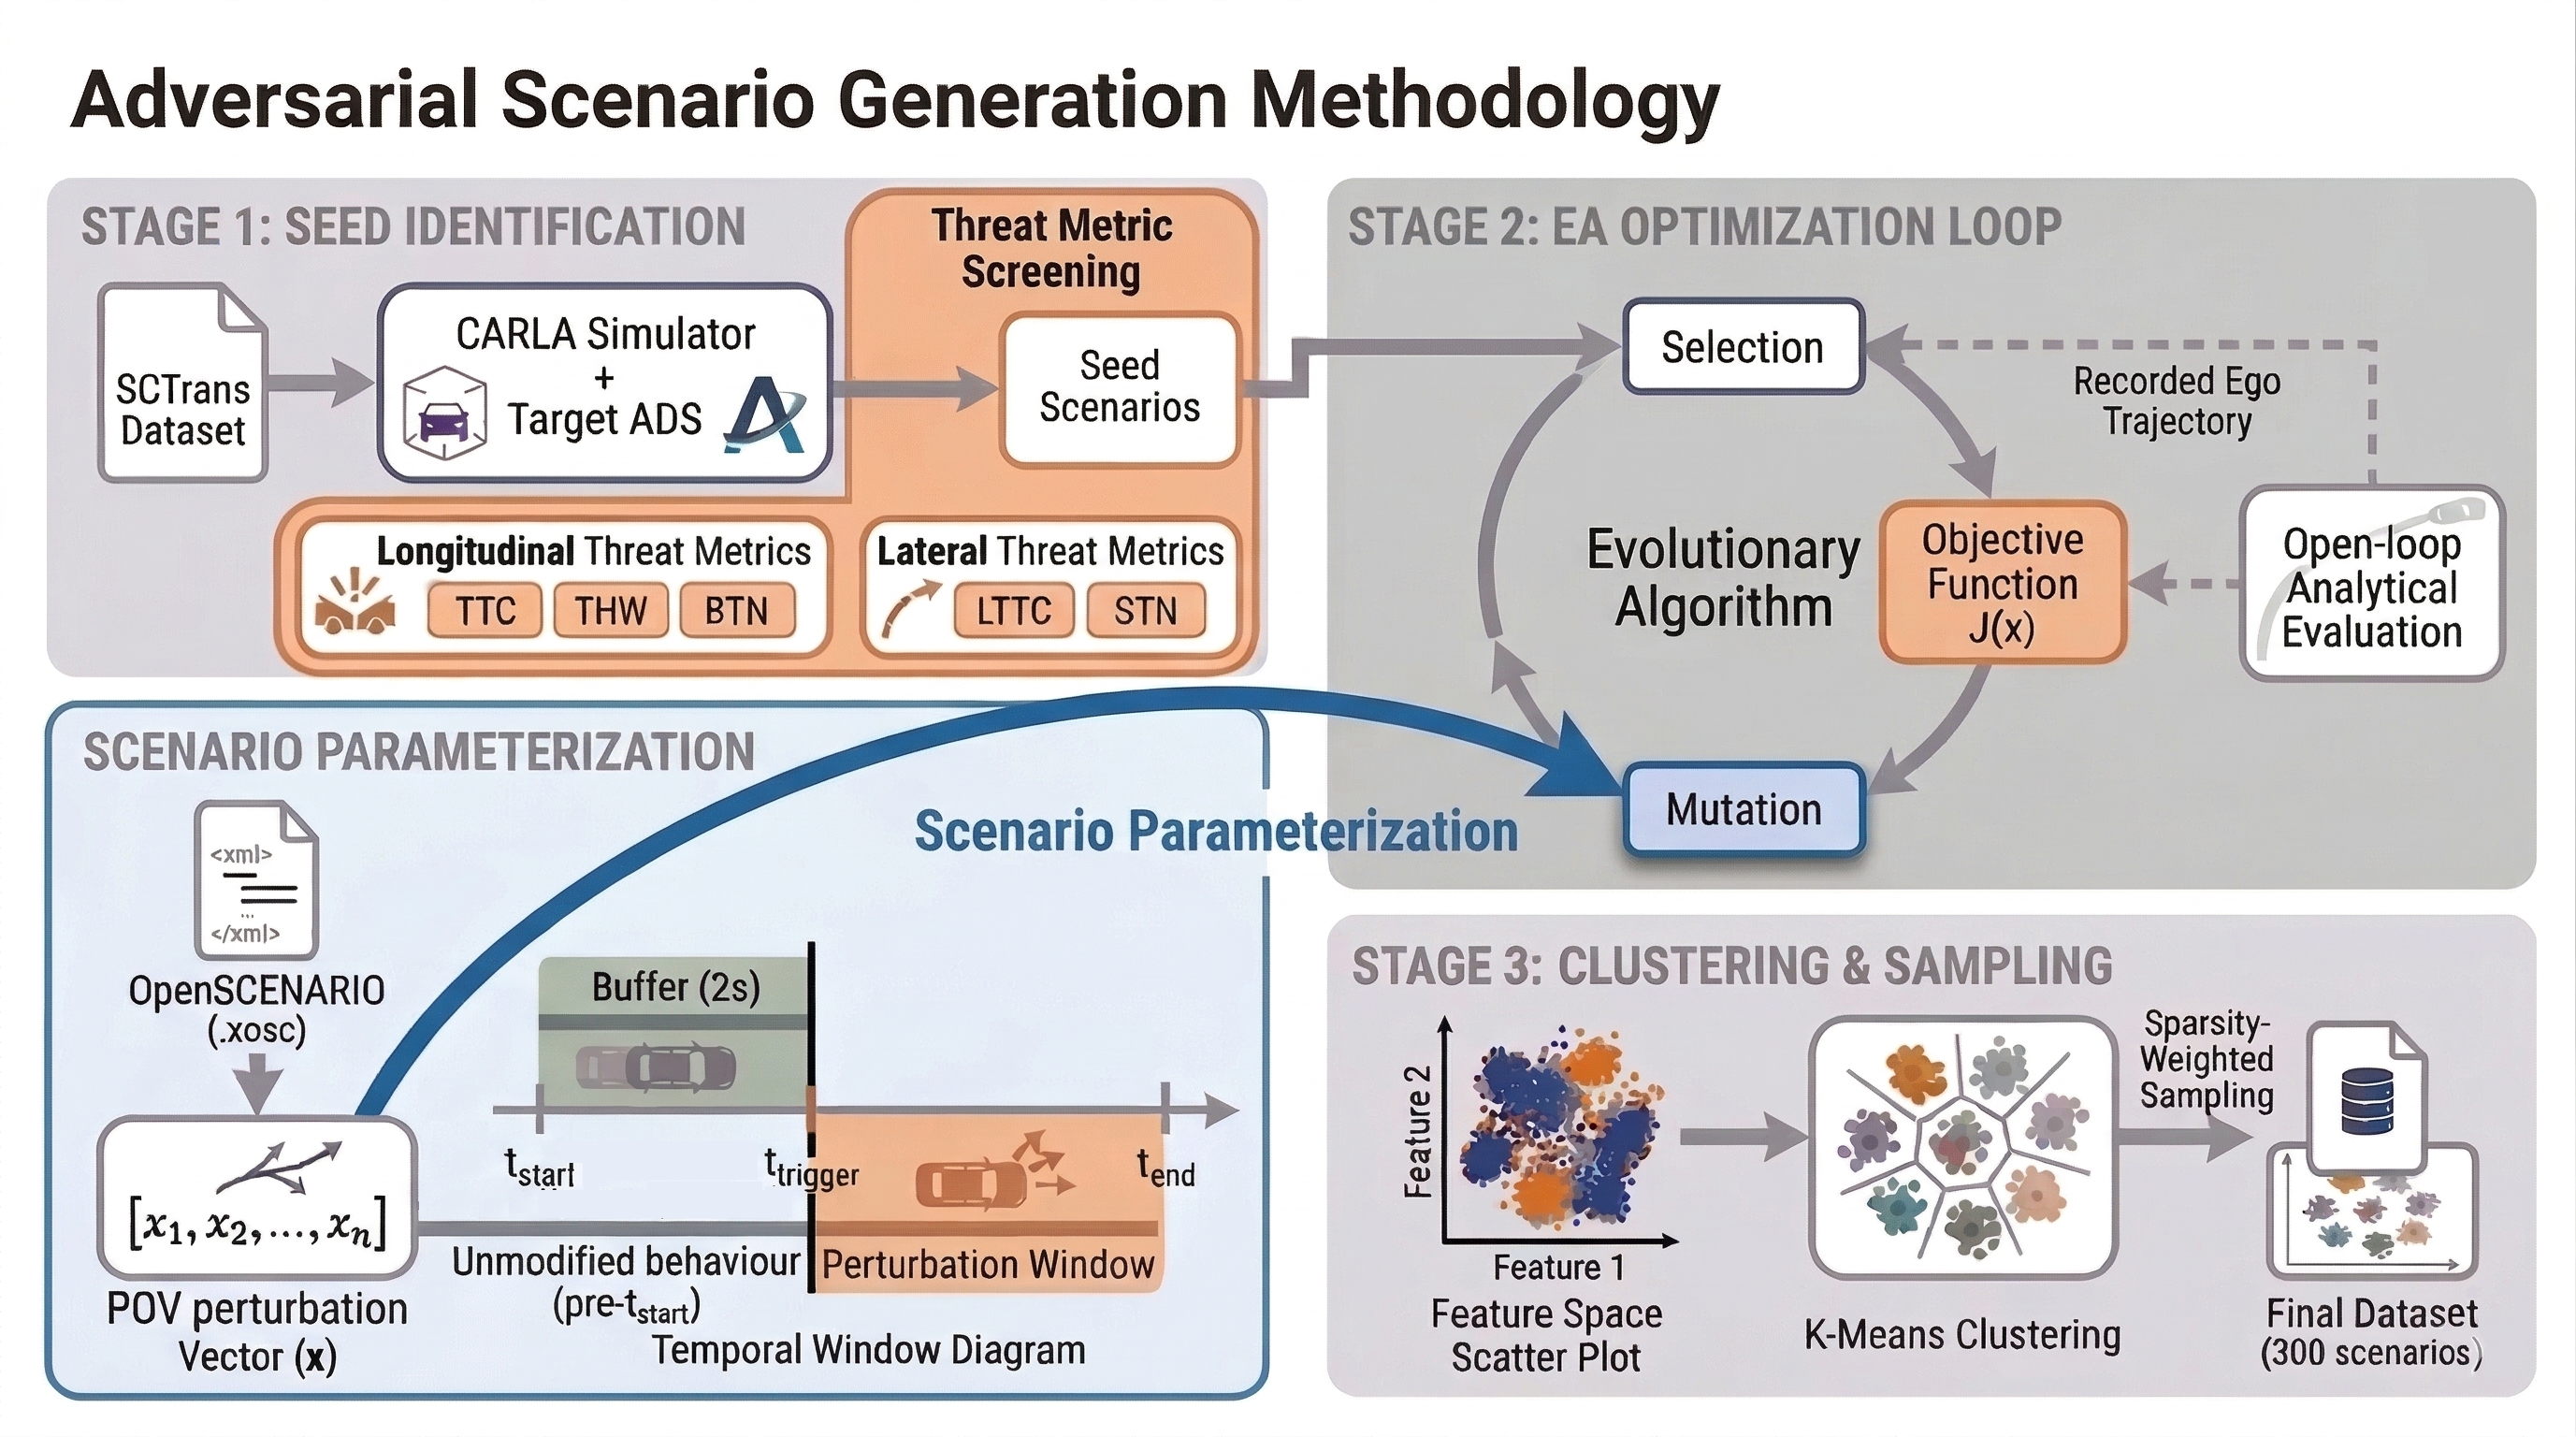
\includegraphics[width=0.8\textwidth]{figures/generation_workflow.jpg}
    \caption{Overview of the adversarial scenario generation pipeline: seed identification via threat metric screening, scenario parameterization with temporal windowing, evolutionary algorithm optimization using open-loop analytical evaluation, and diversity-driven clustering and sampling.}

    \label{fig:generation_workflow}
\end{figure*}

\subsection{Threat Metrics and Threshold Selection}
\label{sec:threshold_selection}
To identify safety-critical scenarios from the broader dataset, we require a principled method for quantifying collision risk during baseline simulations. We employ five kinematic threat metrics grouped by the dominant conflict direction. The metrics and their associated thresholds provide the quantitative foundation for both seed scenario identification and adversarial scenario evaluation.
\subsubsection{Threat Metric Definitions}
\label{sec:threat_metrics}

For longitudinal and junction conflicts, we define three metrics that capture temporal proximity and braking demand. Time-to-Collision (TTC) and Time Headway (THW) measure the temporal margin available to the ego vehicle, while the Brake Threat Number (BTN) quantifies the required deceleration relative to the vehicle's physical braking limit:
\begin{equation}
    \text{TTC} = \frac{x_{rel}}{v_{x, rel}}, \quad \text{THW} = \frac{x_{rel}}{v_{ego}}, \quad \text{BTN} = \frac{a_{x, req}}{a_{x, max}}
\end{equation}
where $x_{rel}$ and $v_{x, rel}$ are the relative longitudinal distance and velocity, $v_{ego}$ is the ego vehicle's speed, $a_{x, req}$ is the required deceleration to avoid collision, and $a_{x, max}$ is the vehicle's maximum physical braking limit. Lower TTC and THW values indicate greater temporal urgency, while higher BTN values indicate greater braking severity. To prevent mathematical instability when $v_{x, rel}$ approaches zero, the upper bounds of TTC and THW are capped at their corresponding critical thresholds as specified in Table~\ref{tab:thresholds}.

For lateral conflicts such as lane changing and drifting, $v_{x, rel}$ approaches zero, rendering TTC mathematically unstable. We therefore substitute the longitudinal metrics with Lateral Time-to-Collision (LTTC) and Steering Threat Number (STN):
\begin{equation}
    \text{LTTC} = \frac{y_{rel}}{v_{y, rel}}, \quad \text{STN} = \frac{a_{y, req}}{a_{y, max}}
\end{equation}
where $y_{rel}$ and $v_{y, rel}$ are the relative lateral distance and velocity, $a_{y, req}$ is the required lateral evasion acceleration, and $a_{y, max}$ is the maximum lateral acceleration capacity governed by road friction limits. The assignment of metrics to kinematic categories follows Table~\ref{tab:kinematic_categories}.

\subsubsection{Threshold Selection}
\label{sec:thresholds}
Each metric is assigned a two-tier threshold structure. The \textit{critical} tier identifies the onset of a safety-relevant interaction and is used to filter baseline simulations for near-miss events that serve as seed scenarios for adversarial generation. The \textit{emergency} tier defines the boundary of an unavoidable conflict and serves as the threat threshold for the optimisation process: candidate scenarios must drive at least one metric beyond its emergency threshold to be retained. The threshold values, summarised in Table~\ref{tab:thresholds}, are derived from the Euro~NCAP Assisted Driving Highway \& Interurban Test and Assessment Protocol v2.2~\cite{noauthor_euro_nodate}.

\begin{table}[htbp]
\centering
\caption{Threat metric thresholds derived from the Euro~NCAP Assisted Driving Highway \& Interurban Test and Assessment Protocol v2.2~\cite{noauthor_euro_nodate}.}
\label{tab:thresholds}
\renewcommand{\arraystretch}{1.0}
\begin{tabular}{@{}llcl@{}}
\toprule
\textbf{Metric} & \textbf{Level} & \textbf{Value} & \textbf{Derivation Basis} \\
\midrule
\multirow{2}{*}{TTC}
  & Critical  & 3.0  & ACC abort criterion (\S3.3.1.1)          \\
  & Emergency & 1.5  & FCW issuance threshold (\S4.3.1)         \\
\multirow{2}{*}{THW}
  & Critical  & 2.0  & ISO~15622 upper bound   \\
  & Emergency & 1.0  & ACC minimum gap (\S3.3.1.1)   \\
\multirow{2}{*}{BTN}
  & Critical  & 0.52 & CCRs (\S3.3.1) \\
  & Emergency & 0.80 & ACC-to-AEB transition (\S4.3.1)   \\
\multirow{2}{*}{LTTC}
  & Critical  & 1.5  & Cut-in TTC (\S3.3.1.3)   \\
  & Emergency & 0.5  & C2MC cut-in TTC (\S3.3.2.5) \\
\multirow{2}{*}{STN}
  & Critical  & 0.40 & Lane Support System (\S4.3.5) \\
  & Emergency & 0.64 & S-Bend (\S3.4.1) \\
\bottomrule
\end{tabular}
\end{table}

Of the ten threshold values, four (TTC critical and emergency, LTTC critical and emergency) are directly mapped from explicitly stated protocol parameters --- test abort criteria, warning issuance deadlines, and prescribed TTC values at lane-change completion. The remaining six are derived from the protocol's test configurations through established physical relationships: THW values from the closest following distance requirement, BTN values from the most demanding ACC scenario (CCRs) and the ACC-to-AEB transition boundary, and STN values from the LKA departure threshold and the S-Bend lateral acceleration demand.

\subsection{Adversarial Scenario Generation -- Regular Setting}\label{sec:generation}
Building on the ten target typologies and their associated threat metrics defined in Sec.~\ref{sec:typology_selection} and~\ref{sec:threshold_selection}, this section presents the adversarial scenario generation pipeline. The core objective is to transform near-miss traffic events into more critical, collision-likely test cases without violating physical plausibility. An overview of the complete pipeline is illustrated in Fig.~\ref{fig:generation_workflow}. The pipeline begins with an empirical screening phase, simulating 854 real-world traffic events from the SCTrans dataset in the CARLA simulator to identify vulnerable ``seed'' scenarios which trigger the predefined threat metrics corresponding to each typology. We frame the adversarial generation as a constrained optimization problem. By parameterizing the dynamic behavior of the Principal Other Vehicle (POV) within the OpenSCENARIO framework and constraining these bounds to Euro NCAP regulatory standards, we maintain strict kinematic realism. An evolutionary algorithm (EA) iteratively perturbs these variables using open-loop analytical evaluation against recorded ego-vehicle trajectories, guided by the typology-specific objective function. A key contribution of this methodology is the open-loop analytical optimization with temporally scoped perturbations (Sec.~\ref{sec:seed}): by restricting modifications to the threat-metric-triggered window and evaluating against recorded baseline trajectories, we achieve efficient search-space exploration while maintaining the physical validity of each generated scenario. Finally, feature-space clustering with sparsity-weighted sampling distills the results into 300 highly diverse, representative failure modes across all ten typologies.

\subsubsection{Seed Scenario Identification and Parameterization}\label{sec:seed}

The adversarial generation pipeline begins with the empirical identification of high-risk baseline events. We execute 854 original, unperturbed scenarios from the SCTrans dataset within the CARLA simulator, utilizing Apollo as the target ego vehicle. During these baseline simulations, we continuously monitor the kinematic interactions between the ego vehicle and the surrounding traffic. Scenarios that breach safe operational thresholds and trigger our target threat metrics (TTC, THW, and BTN for longitudinal conflicts; LTTC and STN for lateral conflicts) are classified as near-misses and extracted as foundational ``seed'' scenarios. The threshold values defining these near-miss boundaries are established in Sec~\ref{sec:threshold_selection}.

Once these vulnerable seeds are identified, their existing OpenSCENARIO (\texttt{.xosc}) definitions are restructured to decouple the static environment from the parameterized adversarial agent. The map topology, defined in the corresponding \texttt{.xodr} files, remains unchanged. Static environmental constraints and background non-POV traffic within the \texttt{.xosc} files are preserved, constrained to their recorded trajectories, to maintain the baseline realism of the SCTrans data. Conversely, the dynamic state of the Principal Other Vehicle (POV)---the primary adversarial agent---is parameterized to form a continuous search space. Crucially, we do not modify the entire scenario timeline. For each seed, we identify the temporal window during which the threat metrics are actively triggered, and restrict perturbations exclusively to this window plus a 2-second preceding buffer. This buffer allows the POV to transition smoothly from its unmodified baseline behavior to the perturbed, higher-risk state. All behavior prior to this window remains identical to the original scenario, ensuring that the ego vehicle's recorded trajectory up to the onset of the perturbation window is valid and unaffected.

We define a perturbation vector $\mathbf{x}$ for each seed, encompassing variables such as the POV's initial velocity ($v_{POV}$) and acceleration profiles ($a_{POV}$). We utilize OpenSCENARIO triggers, specifically the \texttt{RelativeDistanceCondition}, \texttt{RelativeSpeedCondition}, to define the exact spatial and velocity thresholds at which the POV executes risky behaviors, such as a sudden brake within a critical time window when the ego vehicle is trailing, or an aggressive lane change. By directly modifying these parameters within the \texttt{.xosc} XML structure, we create a controllable testbed ready for heuristic optimization.

\subsubsection{Defining the Objective Function}\label{sec:objective}
To guide the search algorithm toward a collision state, we formulate a fitness function $J(\mathbf{x})$ that quantitatively evaluates the danger of each candidate trajectory. The function is designed such that lower values of $J(\mathbf{x})$ indicate higher collision risk, and the evolutionary algorithm seeks to minimize it. The unified objective function is formulated as:
\begin{equation}
    J(\mathbf{x}) = \sum_{i} \mathcal{T}_{i}(\mathbf{x}) - \sum_{j} \mathcal{R}_{j}(\mathbf{x})
\end{equation}
where $\mathcal{T}_{i}(\mathbf{x})$ denotes the time-based proximity metrics (TTC/THW for longitudinal conflicts, or LTTC for lateral conflicts) and $\mathcal{R}_{j}(\mathbf{x})$ denotes the threat number metrics (BTN for longitudinal conflicts, or STN for lateral conflicts), as defined in Sec.~\ref{sec:threat_metrics}. The time-based metrics decrease as collision risk increases, while the threat numbers increase with risk; subtracting the latter ensures that all terms contribute consistently toward a lower $J(\mathbf{x})$ for higher-risk scenarios. All metrics are weighted equally, as they capture complementary aspects of collision risk: temporal margins and the required evasive effort. Minimizing $J(\mathbf{x})$ therefore simultaneously drives the scenario toward shorter time margins and greater difficulty for the ego vehicle to avoid collision.

\subsubsection{Optimization and Search Algorithm}\label{sec:optimization}
We model the generation pipeline as a constrained optimization problem, utilizing an Evolutionary Algorithm (EA) to iteratively evolve the perturbation vector $\mathbf{x}$ toward a critical collision boundary. To ensure that perturbed trajectories remain physically plausible, the allowable boundaries for $\mathbf{x}$ are strictly constrained according to the Euro NCAP AD Test and Assessment Protocol v2.2, ensuring that every generated scenario represents a standardized, kinematically valid testing condition rather than an edge-case simulator artifact. This optimization phase operates entirely through open-loop analytical evaluation rather than closed-loop simulation, enabling efficient and broad search-space exploration.

We use the ego-vehicle trajectory recorded during the preliminary baseline simulation in CARLA. For every candidate generated by the EA, we analytically superimpose the perturbed POV behavior onto this recorded trajectory. As described in Sec.~\ref{sec:seed}, perturbations are restricted to the threat-metric-triggered window and its preceding 2-second buffer, ensuring that the ego vehicle's behavior prior to this window remains identical to the baseline. By evaluating the ego vehicle in this open-loop manner---without factoring in closed-loop evasive responses---the EA is directed toward scenarios that are analytically more critical than the original seeds.

The EA employs a standard evolutionary loop: parent selection is performed across the full candidate pool, and mutation is applied to a sampled 10\% of the population at each generation to introduce controlled variation while preserving the majority of high-fitness solutions. The fitness function $J(\mathbf{x})$ evaluates the analytically superimposed trajectories using the typology-specific threat metrics to quantify the collision risk. The EA selects the parameter combinations yielding the lowest $J(\mathbf{x})$ to breed the next generation, continuously refining the POV's adversarial behavior. The EA terminates once it has collected a sufficient pool of 100 candidate scenarios that surpass at least one threat threshold for each typology. This threshold serves as a quality floor, ensuring all retained scenarios represent a meaningful increase in risk over their original seeds, while preserving diversity in the solution space for the subsequent clustering stage. The specific threat threshold values are detailed in Sec.~\ref{sec:threshold_selection} and Sec.~\ref{sec:objective}.

\subsubsection{Clustering and Selection}
Once the evolutionary algorithm produces a large pool of high-risk candidates, we distill these results into a highly diverse, non-redundant dataset. For each of the ten NHTSA typologies, the EA generates a pool of 100 candidate scenarios, each surpassing the predefined threat threshold. We then extract the kinematic features of each scenario at the point of highest threat, such as the relative speed, approach angle, and required ego-vehicle deceleration. Unlike the threat metrics used in the fitness function, which quantify pre-crash risk during optimization, these features characterize the physical crash outcome and are therefore better suited for distinguishing between structurally different failure modes. For each typology, these features are mapped into a multi-dimensional feature space and grouped using a K-Means clustering algorithm based on physical and kinetic similarity. To select the 30 representative scenarios per typology, we employ sparsity-weighted sampling: the algorithm probabilistically favors scenarios with greater distance to their nearest neighbor in feature space. This per-typology process yields a final dataset of 300 scenarios (30 $\times$ 10 typologies) that captures a wide spectrum of failure modes while avoiding redundant crash dynamics.
